% (opsional) gunakan penomoran romawi untuk front matter
\pagenumbering{roman}

% --- COVER ---
% Jika Anda punya cover.pdf (1 halaman)
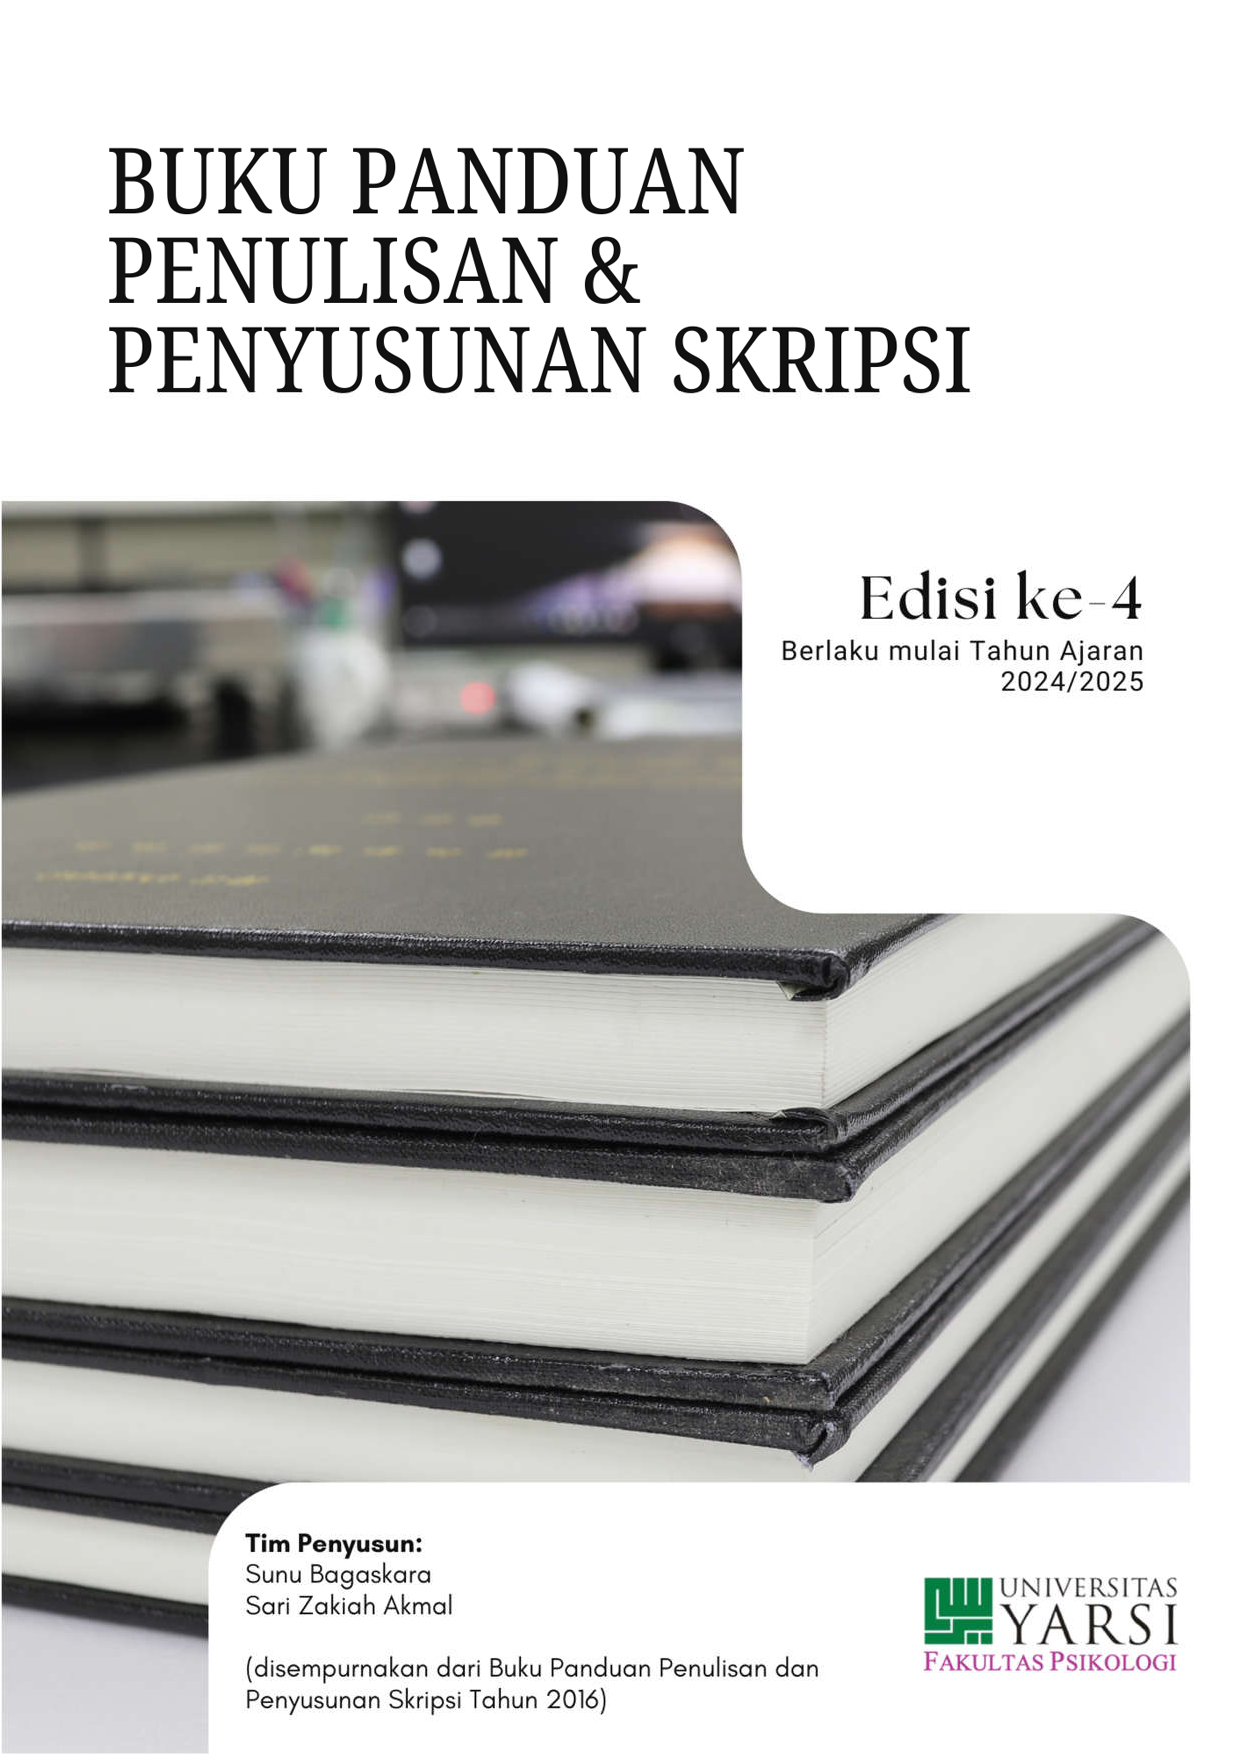
\includepdf[pages=1,fitpaper=true]{cover.pdf}
\cleardoublepage

% --- HALAMAN JUDUL ---
\begin{titlepage}
\centering
\vspace*{2.5cm}
{\fontsize{22pt}{26pt}\selectfont\bfseries Buku Panduan\\[2mm]}
{\fontsize{22pt}{26pt}\selectfont\bfseries Penulisan \& Penyusunan Skripsi\par}

\vspace{1.2cm}
\rule{\linewidth}{0.5pt}\\[-6pt]
{\large \textbf{Fakultas Psikologi Universitas YARSI}}\par
\rule{\linewidth}{0.5pt}

\vspace{1.4cm}
{\large \textbf{Edisi Ke-4}\par}

\vfill
{\large \textbf{Tim Penyusun:}}\par
{\large Sunu Bagaskara\par}
{\large Sari Zakiah Akmal\par}
\vspace*{1.2cm}
\end{titlepage}
\cleardoublepage

% --- BALIK HALAMAN JUDUL (verso) ---
\thispagestyle{empty}
\vspace*{\fill}
\begin{center}
\textit{Buku Panduan Penulisan \& Penyusunan Skripsi}\\
Fakultas Psikologi Universitas YARSI\\[6pt]
Hak Cipta © 2025 Fakultas Psikologi Universitas YARSI\\
ISBN: (isi bila ada)
\end{center}
\vspace*{\fill}
\clearpage